\chapter*{}

\vfill
{\itshape
\lipsum[2]
}

\chapter*{Bava \frank{א}
\smallskip\subtitulo{Passado}}
\addcontentsline{toc}{chapter}{\textsc{bava} {\frank א}
\quad Passado}

\begin{center}
{\huge\brabo{
\textit{As perspectivas de um portão}
}}\\\medskip{\footnotesize\formularlight{
É na travessia de um limite que realmente se percebe o cenário em volta. Mas esse marco, que anuncia um ponto de observação, não diz respeito à experiência em si. O observador, personagem-forasteiro que cruza a fronteira, precisa estar distante o suficiente para agir. Ou compreender. São a tradição e a memória que compõem o arcabouço possível rumo ao outro lado da linha. Como uma tocha que inflama na ventania, o passado guia o desconhecido. Tudo, então, se torna passado: um portão que se abre, um corredor cheio de portas, uma fechadura sem chave. No lusco-fusco entre dois mundos, o movimento não é perceptível.
}}
\end{center}

\paragraph{Os 3 livros} São os modos pelos quais a criação acontece: \textit{sêfer}, o ``livro'', \textit{sefar}, o ``número'' e \textit{sipur}, a ``narrativa''.

\paragraph{As 6 direções cardeais} São cósmicas, e representam camadas da realidade. 

\paragraph{As 10 «sefirót»} São emanações divinas que estruturam \textit{olam}, o ``mundo'', \textit{shaná}, o ``tempo'' e \textit{nefesh}, o ``homem''. Elas se relacionam com os 10 números.
% Elas permitem ao \textit{ein sof}, o ``ilimitado'', se tornar mundo.
% \textit{blimá}, ou ``vindas do vazio''

\paragraph{As 22 letras} São as letras do alfabeto hebraico, forças arquetípicas que estruturam tudo o que existe.
% Instrumentos de criação.

\paragraph{As 3 letras mães} \textls[-5]{Funcionam como um eixo, uma balança. Os pilares da existência. Estão em perfeito equilíbrio e representam os elementos primordiais: fogo, relacionado à cabeça; ar, relacionado ao tórax; e água, relacionada à barriga. O ar, elemento intermediário e que equilibra o fogo que sobe e a água que desce, equivale a 3 aspectos humanos: \textit{nefesh}, a ``respiração'', \textit{ruach}, o ``espírito'' e \textit{neshamá}, a ``expiração''. A terra e o éter, que estão abaixo ou acima de nós, não são citados na literatura do \textit{Sêfer Ietzirá}.}

\paragraph{As 7 letras duplas} São compostas pelo masculino e pelo feminino, \textit{zachar unekevá}, as polaridades do mundo. E essa duplicidade é navegável. Representam os dias da semana e os 7 planetas clássicos: Sol, Lua, Marte, Mercúrio, Júpiter, Vênus e Saturno.

\paragraph{As 12 letras simples} Representam as variações e ciclos da existência. Se relacionam com os 12 órgãos condutores na \textit{alma-corpo}, os 12 signos do zodíaco e os meses do ano.

\paragraph{Os 32 caminhos de sabedoria} \textls[15]{Reúnem as 22 letras do alfabeto hebraico e as 10 sefirót. São os caminhos de como a criação se manifesta.}

\paragraph{Os 231 portões} \textls[-15]{Dizem respeito a todas as combinações possíveis entre as 22 letras do alfabeto, considerando pares não repetidos e sem reversão. Ou seja, todos os sons hebraicos possíveis. Compreendem tudo o que se encontra no mundo, no tempo e no homem.}

% A realidade, que é feita de relações e combinações, está sempre em transformação. Ao mudar, cria-se algo novo. Cada par de letras representa, portanto, um portão de som e de sentido: a ligação entre duas ideias, dois sons, duas forças. Quando combinadas ou intercambiadas, essas letras geram vibrações ou expressões de princípios cósmicos. E torna-se possível \textit{tocar} o ato criador. 

% Os portões sonoros guardam essas travessias. Cada som que existe foi um combinado de letras no tempo. E nada que foi dito ou feito desaparece. São portões de transição únicos. Mas, ao mesmo tempo, qualquer combinação permite novas recombinações. O passado é um reservatório de possibilidades e novos sentidos.}

%\pagebreak

\begin{figure}[htpb!]
\thispagestyle{empty}
\vspace*{-2cm}
\hspace*{-2.5cm}
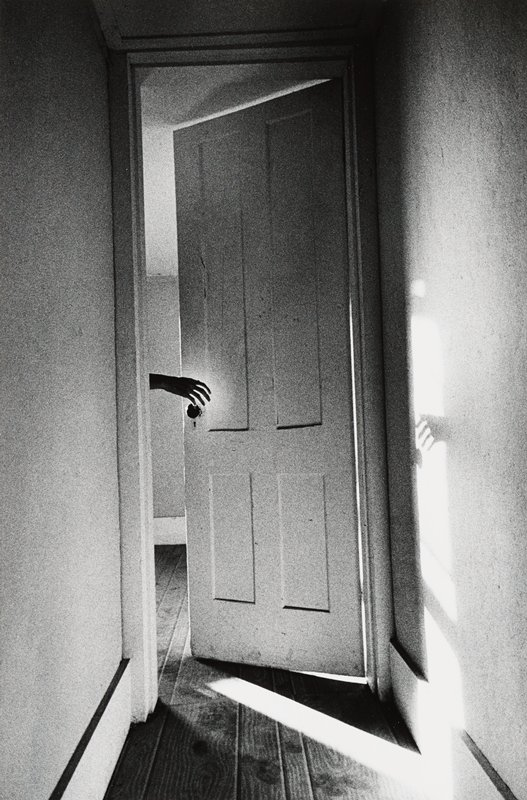
\includegraphics[width=1.5\textwidth]{./IMAGEM.jpg}
\end{figure}

\pagebreak
{\pagecolor{black}}
\mbox{}
\pagebreak
\afterpage{\nopagecolor}

\chapter*{Bava \frank{ב}
\smallskip\subtitulo{Serpente}}
\addcontentsline{toc}{chapter}{\textsc{bava} {\frank ב}
\quad Serpente}

% Conhecimento
\begin{center}
{\huge\brabo{
\textit{O «frisson» de conhecer}
}}\\\medskip{\footnotesize\formularlight{
O brilho de um relâmpago\footnote{A única descrição sobre o aspecto das dez \textit{sefirót} que consta no \textit{Sêfer Ietzirá} é que são, traduzindo livremente do hebraico, ``como o brilho de um relâmpago, e que seu fim não tem limite''. O estilo fragmentário do texto, em aforismos ou \textit{mishnaiót}, evocam um estilo que tende a dar forma às revelações.} é uma constelação de perdas e encontros, na qual as revelações se dão descontínua e repentinamente. Esses instantes de verdade podem, por um instante, se iluminar. E os vislumbres são também rompimentos, pois são vivos e pulsantes: por mais que vindos do passado, interpelam o presente. Em desafio à linearidade e à ideia de progresso, só podem ser percebidos pelos que têm o olhar desperto. Cabe ao pensamento, à escrita ou à leitura captar essas cintilações efêmeras, que mostram indiretamente uma verdade encoberta. Como um campo em ruínas onde ainda brilham centelhas dispersas, a verdade não se dá por totalidade, mas por irrupção.
}}
\end{center} 

\paragraph{A descoberta se parece com a completude} A \textit{alegria de conhecer}, segundo Hasdai Creskas, acontece quando se compreende a criação. E o conhecimento, que é carregado de afeto, provoca intensa alegria, algo que ultrapassa a razão.\footnote{\textls[20]{Maimônides, diferente de Creskas, vê a alegria intelectual como uma consequência da perfeição racional.}} Conhecer não é apenas entender, mas sentir. Como diz Gersônides, Deus não é feliz por conhecer tudo, mas feliz com a criação. Todo conhecimento genuíno revela algo sobre Deus. E isso gera alegria.

\paragraph{Viver e significar} É uma experiência racional e existencial. E se, para o Deus de Creskas, amor é união, a força entre o humano e o celeste é a percepção da verdade divina na vida cotidiana.

\paragraph{Conhecer e relacionar} Para Buber é impossível \textit{conhecer alguém} no sentido literal da palavra. Conhecer (\textit{eu--isso}) envolve estudo, análise e observação. Ao conhecer, objetifica-se o outro. Relacionar-se (\textit{eu--tu}), por outro lado, é o encontro genuíno, quando as duas partes se abrem ao diálogo. 
% Relacionar-se é uma experiência de vivência.

\chapter*{Bava \frank{ג}
\smallskip\subtitulo{Encanto}}
\addcontentsline{toc}{chapter}{\textsc{bava} {\frank ג}
\quad Encanto}

% Criação
\begin{center}
{\huge\brabo{
\textit{Os sábios podem criar mundos}
}}\\\medskip{\footnotesize\formularlight{
\lipsum[2]
}}
\end{center}

% \setlength{\epigraphwidth}{.60\textwidth}
% \begin{epigraphs} 
% \qitem{Se os justos quisessem, poderiam criar mundos, pois está escrito: \textit{Mas os vossos pecados fazem separação entre vós e o vosso Deus.}}{\textsc{isaías 59--2}}
% \qitem{Rava disse: ``Se os justos desejassem, poderiam criar um mundo, pois é dito sobre Bezalel: \textit{Ele sabia como combinar as letras com as quais os céus e a terra foram criados.''}}{\textsc{sanhedrin 65b}} 
% \end{epigraphs}

\paragraph{Linguagem criativa} Ao dominar o conhecimento da articulação de letras, sons e números, como foi feito por Deus segundo a Torá, é possível gerar mundos. Mas, na tradição cabalística, não se trata apenas de pronunciar palavras. É preciso entender como esses mundos se relacionam e se combinam: criação é formatação. No \textit{Sêfer Ietzirá}, a criação não acontece \textit{ex-nihilo},\footnote{Expressão latina que significa literalmente ``a partir do nada''. É uma maneira de entender a criação similar ao pensamento estoico, que entende o universo como um processo de ordenação e transformação da matéria existente através do \textit{logos}, o princípio racional ativo que organiza o caos em cosmos.} mas através da combinação e manipulação de forças que já existem.

\paragraph{Betzalel «sabia como combinar as letras»\footnote{Referência à passagem do Talmud, do tratado Berachot. Trata-se de um elogio à sabedoria de Betzalel, o artífice escolhido para construir o Mishkan, um templo móvel construído sob orientação direta de Deus a Moisés.}} Betzalel, que podia criar \textit{formas espirituais} no mundo material, conhecia os segredos da criação por meio das letras. Ele traduzia os códigos divinos para uma realidade sensível. Suas obras não eram apenas objetos belos e funcionais, mas resonâncias físicas de ordens invisíveis. Ele moldava ouro e madeira como quem pronuncia um nome sagrado.

\paragraph{Criação é um processo eterno} As letras hebraicas são entendidas como elementos fundamentais, semelhantes aos princípios ativos da filosofia estoica.\footnote{O fogo, o ar e a energia vital, o \textit{pneuma}.} Através dessas forças cósmicas e dinâmicas, o mundo fica sujeito a constante transformação. E esse conceito ecoa em várias práticas, como o estudo e a interpretação da Torá --- uma contínua obra de criação ---, ou escolas de pensamento --- como, por exemplo, a psicanálise, que surgiria muitos séculos depois.

\chapter*{Bava \frank{ד}
\smallskip\subtitulo{Sonho}}
\addcontentsline{toc}{chapter}{\textsc{bava} {\frank ד}
\quad Sonho}

% Criação e psicanálise
\begin{center}
{\huge\brabo{
\textit{Os significados ocultos}
}}\\\medskip{\footnotesize\formularlight{
\lipsum[2]
}}
\end{center}

\paragraph{A realidade não é fixa} Constantemente interpretado e reinterpretado por meio de símbolos, o mundo é entendido como dinâmico para a tradição cabalista e psicanalítica. Assim como no \textit{Sêfer Ietzirá}, onde o mundo é recriado constantemente pelas combinações das letras, o inconsciente psicanalítico reorganiza símbolos, memórias e significados como um processo de construção contínua, que cria e recria a realidade psíquica do sujeito. 

\paragraph{Partes perdidas de si} \textls[15]{A ideia de criação contínua no \textit{Sêfer Ietzirá} se conecta ao \textit{Tikun Olam}, que sugere que o universo está em constante processo de correção e aperfeiçoamento. Para Winnicott, por exemplo, o processo terapêutico é visto como um espaço de criação onde o paciente se redescobre e reconstrói sua identidade. Tanto o \textit{Sêfer Ietzirá} quanto a psicanálise acreditam que \textit{saber falar é saber criar}.}

\paragraph{Criação e Torá} \textls[15]{Zohar, um dos livros mais importantes da mística judaica, diz que ``Deus olhou para a Torá e criou o mundo''. A Torá, aqui, não é entendida apenas um texto religioso --- mas uma estrutura dinâmica da realidade, parecida com o \textit{logos} no pensamento estoico. Cada letra, palavra e verso tem potencial criativo, e pode ativar forças cósmicas.}

\paragraph{Interpretar é o oposto de decorar} Interpretar a Torá não é apenas extrair o significado literal, mas descobrir os significados ocultos através de técnicas como \textit{midrash}, \textit{gematria} e \textit{notarikon}.\footnote{Acrósticos e combinações de letras.} Assim como o texto da Torá é interpretado de geração em geração, o mundo físico é continuamente reinterpretado e recriado. E o estudo da Torá é parte desse processo. Quando um sábio encontra uma nova interpretação, ele altera a realidade.

\paragraph{Criação e vazio} \textls[20]{O mundo antes da criação formal, no contexto bíblico, é \textit{tohu vavohu}. Mas não é apenas ``vazio''; é um vazio cheio de potencial. É a matéria bruta primordial que contém todas as possibilidades da criação. As letras hebraicas no \textit{Sêfer Ietzirá} são como ``sementes'' de potencial. Antes de serem combinadas, elas existem em um estado \textit{tohu}, ou seja, potencial bruto, sem forma. Quando Deus as combina, elas dão origem ao mundo como o conhecemos.}

\paragraph{O vazio e o caos não são negativos} Lacan diz que a criação de significado está diretamente ligada ao \textit{vazio estrutural no centro do sujeito}. Assim como Deus cria o vazio no \textit{tzimtzum}, o ser humano vive com um vazio interno --- uma falta estrutural que impulsiona o desejo e a busca por sentido. Esse estado é análogo ao \textit{tohu vavohu} porque é um estado dinâmico: não é apenas uma ausência, mas o lugar onde o significado pode ser criado e recriado. O mundo, portanto, está em ato. E ele acontece, segundo o \textit{Sêfer Ietzirá}, em sistema de correspondências.

\chapter*{Bava \frank{ה}
\smallskip\subtitulo{Eva}}
\addcontentsline{toc}{chapter}{\textsc{bava} {\frank ה}
\quad Eva}

% Correspondência; Uma teia interligada
\begin{center}
{\huge\brabo{
\textit{Atuo aqui e causo efeito lá}
}}\\\medskip{\footnotesize\formularlight{
\lipsum[2]
}}
\end{center}

\paragraph{Correspondências simbólicas} \textls[-15]{A principal ideia da magia é a brincadeira com as noções de microcosmo e macrocosmo. Na visão mágica, o universo é como uma teia interligada. E o praticante não cria algo estritamente novo, mas reorganiza o fluxo de energias existentes. A correspondência sugere que há uma relação simbólica entre diferentes planos da realidade: espiritual, mental e físico. Planetas estão associados a emoções humanas, ervas podem estar conectadas a deuses, e números podem refletir qualidades divinas. Na astrologia, cada planeta é associado a cores, metais e plantas.} %Para atrair amor e harmonia, é indicado um ritual associado a Vênus usando objetos como cobre, rosas e a cor verde --- pois todos esses elementos correspondem ao domínio desse planeta.

\paragraph{A essência comum} \textls[10]{Ao entender as relações entre os diferentes planos, é possível manipular símbolos para gerar mudanças nos planos superiores e vice-versa. As correspondências são o código que traduz a vontade do mago em efeitos concretos. E são o que pressupõe o universo como um todo interligado: o que acontece em uma parte dele pode influenciar outras.}

\paragraph{O gatilho} O nome de Eva, ou Chava, vem de \textit{chai}, ``vida''. Mas sua figura não representa apenas a mãe de todos os seres humanos, a que ``dá a vida'' --- mas o próprio canal da existência e da transformação. Enquanto Adão, ou Adam, está associado à \textit{adamá}, ``terra'', à estrutura e à estabilidade, Eva representa o fluxo da experiência e o princípio dinâmico de criação. Ela perfurou a realidade do Éden e viu o que estava oculto. Com isso, abriu um novo caminho de consciência: através de uma ação, tudo mudou. %É a ideia cabalística de que o que ocorre aqui reverbera nos mundos superiores.

\paragraph{A transgressão} No judaísmo, o entendimento profundo não é relacionado à obediência, mas à experiência, à queda e à \textit{teshuvá}, o ``retorno''. O que Eva fez ao comer do fruto pode ser visto como o momento em que a humanidade entrou no mundo da experiência e da ação. Foi o nascimento da consciência.
%Essa separação foi necessária para que houvesse autoconsciência e livre-arbítrio.

\chapter*{Bava \frank{ו}
\smallskip\subtitulo{Silêncio}}
\addcontentsline{toc}{chapter}{\textsc{bava} {\frank ו}
\quad Silêncio}

% Som
\begin{center}
{\huge\brabo{
\textit{A vibração em potência}
}}\\\medskip{\footnotesize\formularlight{
\lipsum[2]
}}
\end{center}

\paragraph{Um tratado sobre o som} \textls[10]{No \textit{Sêfer Ietzirá} não são apenas os números e as letras que importam, mas suas articulações: quando o som molda a estrutura da realidade. Os \textit{231 portões}, uma das principais ideias do livro, descrevem as combinações possíveis entre as 22 letras do alfabeto hebraico. Esses portões simbolizam a união de letras em som e, consequentemente, palavras. O diagrama frequentemente utilizado para representar esse conceito é o \textit{galgal hashe'arim} ou ``roda dos portões'', onde todas as combinações possíveis de letras estão interligadas, formando um sistema de criação dinâmico. Essa ``roda'' também representa o universo e o tempo como tecidos cíclicos.}

\paragraph{Som e respiração} \textls[-15]{Tanto a ideia de um universo dinâmico quanto do som como linguagem que vibra estão ligadas à respiração. O ``sopro'' ou \textit{ruach} remete à energia divina criadora, conforme a criação descrita no Bereshit. E, claro, à vida. Na fala, aliás, o som não existe sem a respiração. São dois movimentos normalmente sincronizados. Isso explica por que a poesia, os cantos religiosos e a música têm efeitos emocionais profundos: eles estão diretamente ligados à modulação do ritmo respiratório. Os mantras recitados em muitas tradições, como o \textsc{om} hindu, ajustam o padrão respiratório para induzir estados meditativos e alinhar mente e corpo.}

\paragraph{O molde da criação} É por meio das letras que esse sopro é ``talhado'' em unidades específicas, permitindo a formação de palavras, que dão forma ao mundo. E as palavras só estão em movimento quando são ditas. Talvez seja justamente por isso que as vogais, que nada mais são do que sons alongados das consoantes, são chamadas em hebraico de \textit{tnuot} ou ``movimento''.

\paragraph{Som potencial} O silêncio, por outro lado, é um espaço latente onde o som está por emergir. Antes de ser moldado em palavras, o sopro está em estado puro, semelhante ao silêncio. Nesse \textit{silêncio primordial} todos os sons possíveis existem e aguardam a ativação pelas combinações de letras. Ele pode ser comparado ao \textit{tohu vavohu} na medida que contém o potencial criador bruto, mas ainda não articulado, ou ao \textit{ein sof}, o estado anterior à manifestação. O nome de Deus, não à toa, é impronunciável.

\chapter*{Bava \frank{ז}
\smallskip\subtitulo{Estrangeiro}}
\addcontentsline{toc}{chapter}{\textsc{bava} {\frank ז}
\quad Estrangeiro}

% Nomes; A luz escreve o sentido
\begin{center}
{\huge\brabo{
\textit{A rebelião conta o destino}
}}\\\medskip{\footnotesize\formularlight{
\lipsum[2]
}}
\end{center}

\paragraph{O mundo é um livro sendo escrito} Os números regulam e as letras são forças cósmicas ativas: esses elementos são como códigos genéticos que produzem organismos e alteram a realidade. E a narrativa é o produto disso. O nome, por outro lado, é a parte da realidade que pode ser definida: no sentido de \textit{dar forma}, \textit{formar}, \textit{formação}. E há um \textit{midrash} importante sobre isso.

\paragraph{O que dizem as estrelas} Abraão, o patriarca, era um grande conhecedor da astrologia antiga, que também incluía astronomia, e sabia interpretar os sinais celestes. Inicialmente, os astros lhe revelaram que ele não poderia ter filhos, mas essa previsão foi alterada através da intervenção divina, marcada simbolicamente pela adição de uma letra ao seu nome. Ao receber a letra {\frank ה} (\textit{hei}) de Deus, ele transcendeu uma limitação. Avram, que se torna Avraham, não é o único. Sarai, sua esposa, também se torna Sara. No \textit{Sêfer Ietzirá}, o \textit{hei} está associado ao elemento ar, ao fôlego (e, como já foi dito, à criação e ao poder vital). É como se a própria essência do ``sopro divino'' fosse incorporada ao nome de Abraão, dando-lhe a capacidade de gerar sua própria linhagem.

\paragraph{Nomes de Deus são ações} Os nomes de Deus não são apenas identificações estáticas, mas expressam as ações, atributos e modos pelos quais Deus se manifesta no mundo. No contexto do \textit{Sêfer Ietzirá}, isso está ligado à criação e ao funcionamento do universo por meio das dez \textit{sefirót} e das combinações das letras hebraicas. Assim, Deus não apenas ``é'' através de seus nomes, mas ``faz'' através deles. Em última análise, os nomes de Deus representam a ponte entre o mundo divino e o mundo material.  

\paragraph{Códigos interrompidos} \textls[-15]{Da mesma forma que Deus não é um nome fixo, o estrangeiro, sempre em trânsito e sem um destino certo, também nunca ``é'' completamente. Para Jean-Luc Godard --- que, por conta da comunicação falha e planos fragmentados, parece operar seu cinema como um idioma estrangeiro ---, o estrangeiro é, aliás, o personagem que desestrutura o discurso. Que traz o desconcerto e a novidade. Ele está fora da gramática dominante, não pertence aos códigos estabelecidos da linguagem e da narrativa e interrompe o fluxo esperado dos significados. É um espectador perdido dentro do filme e, nesse sentido, um revolucionário.}